\documentclass{article}
\usepackage[utf8]{inputenc}
\usepackage{amsmath}
\usepackage{amsfonts}
\usepackage{graphicx}

\title{Stochastic Processes}
\author{Grant Smith }
\date{Spring 2022}

\begin{document}

\maketitle

\section{Introduction}

I want to develop a little intuition between how we think about stochastic processes, for example, the stock market, and how they're defined in a probability book.  First of all, here is a picture:

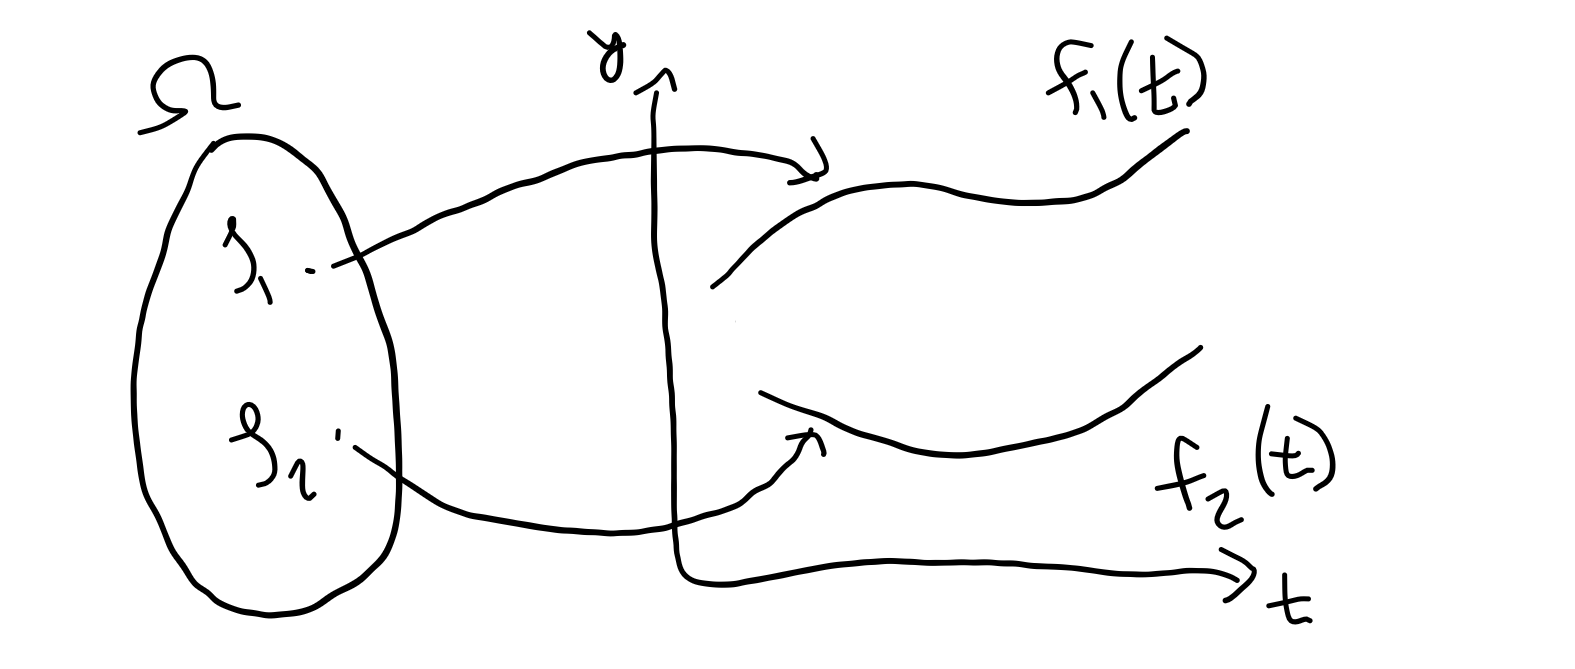
\includegraphics[width=\textwidth]{stochastic_ image.png}

We have a sample space, $\Omega$, and from that sample space, we map to functions of time (or anything else you want).  We call it a stochastic process, but all it is is a function from a sample space to a space of functions.  The notation is $X_t$, but what's under the hood is the following:

$$X_t = x : \Omega \rightarrow \left(\mathbb{R}^+ \rightarrow  \mathbb{R} \right)$$ 

But we don't really perceive that sample space.  What we perceive (for example when observing the stock market) is that we've observed a process up to a certain time, and we don't know what's going to happen next.  How does that fit into the framework above? Let's start with a picture of a stochastic process.  Here it is, and ignore the 3.5 for now. We'll use it in about two paragraphs.

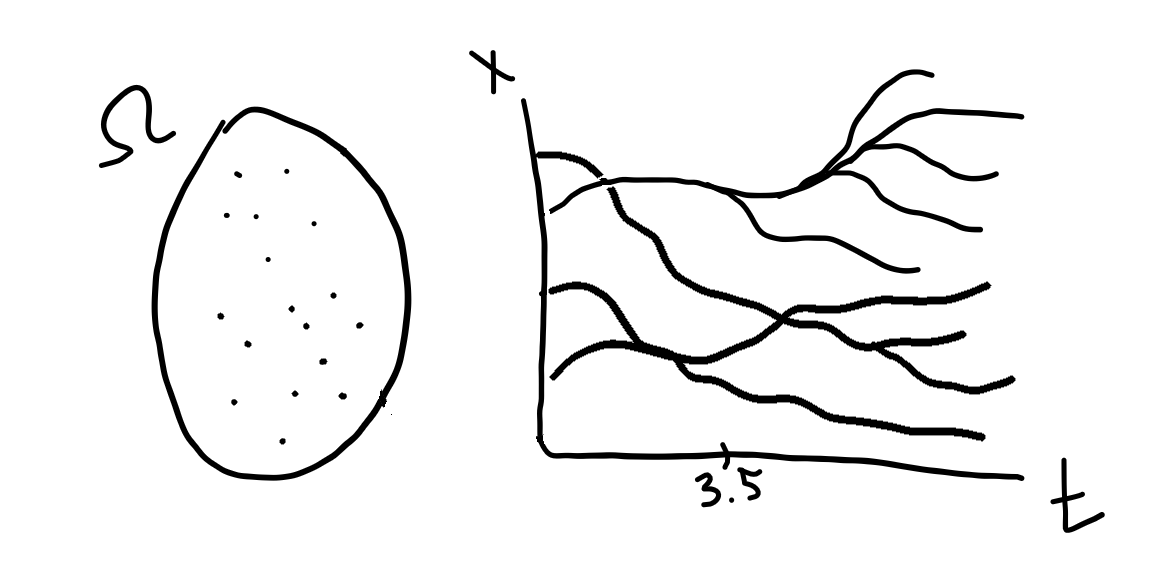
\includegraphics[width=\textwidth]{filtration_part_1.png}

Let's say this is a stock price over time, and we'll call it $X_t$.  The picture on the right is all the possible trajectories, and the sample space on the left has a corresponding event for each trajectory (I didn't count, so the dots and the trajectories probably don't align, but that's okay).

At our initial time, we have no idea which of these trajectories the stock will take.  But then let's wait a little bit (wait until time 3.5) and observe the price.  Let's say the trajectory we observe is the following:

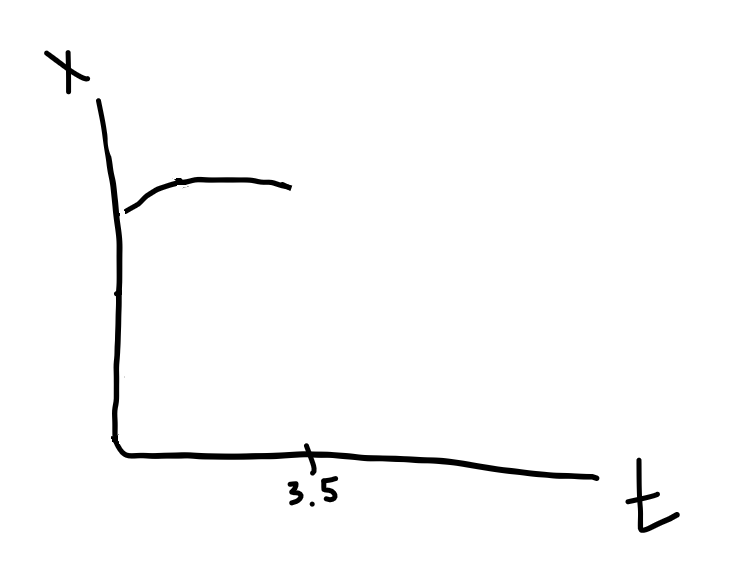
\includegraphics[width=\textwidth]{filtration_part_2.png}

So now we have information about which of the original trajectories are still possible, and which ones are impossible. This is called a filtration, and in our case, we have the filtration at time 3.5, so we will call it$\mathcal{F}_{3.5}$, but in general, it would be $\mathcal{F}_{t}$.

So now we want to figure out what happens to our stochastic process $X_t$ given the information (aka filtration) we know at time 3.5. What the filtration does is filter out all the trajectories that cannot be the case, and it leaves in all the remaining possible trajectories.  The picture is:

\includegraphics[width=\textwidth]{filtration_part_3.png}

You'll notice that the trajectories that don't align with our filtration are gray, and the events in the sample space that correspond to those trajectories are also gray.  And the trajectories that are possible are still black, and their corresponding events are also still black.

This should feel like a conditional probability, and that's exactly what's happening. We want $Y_t := X_t | \mathcal{F}_{3.5}$.  Thus, $Y_t$ is given by the following drawing:

\includegraphics[width=\textwidth]{filtration_part_4.png}

At this point, we've really explained a lot.  One last part you might be wondering is what would happen if we changed the 3.5.  And you'd be right. So our $Y_t$ is dependent upon our observation duration. So I'll ammend our notation to be $X_t(s) := X_t | \mathcal{F}_{s}$, which means that the stochastic process we get (a.k.a. remaining trajectories) depends on how long we observe.  So we could say that $Y_t = X_t(3.5)$.  So let's draw another picture for another time, say 4.5. We will start with what we've observed by time = 4.5:

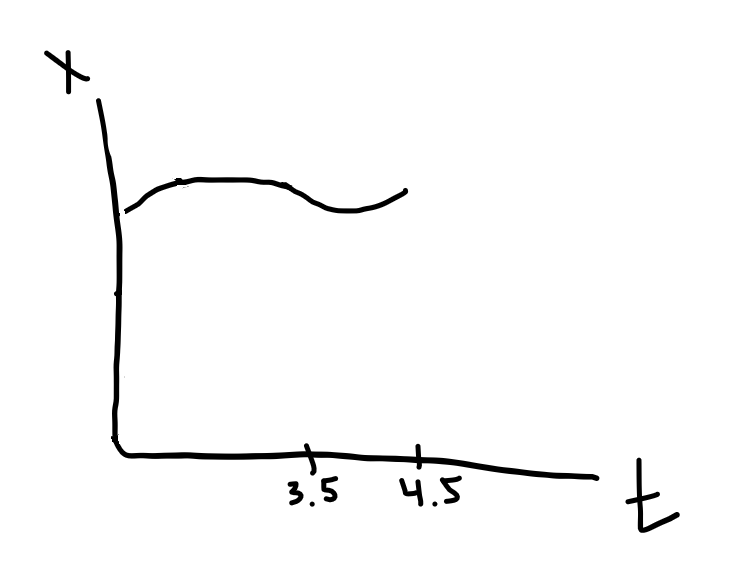
\includegraphics[width=\textwidth]{filtration_4.5.png}

And now we can gray out from the picture of $X_t(3.5)$:

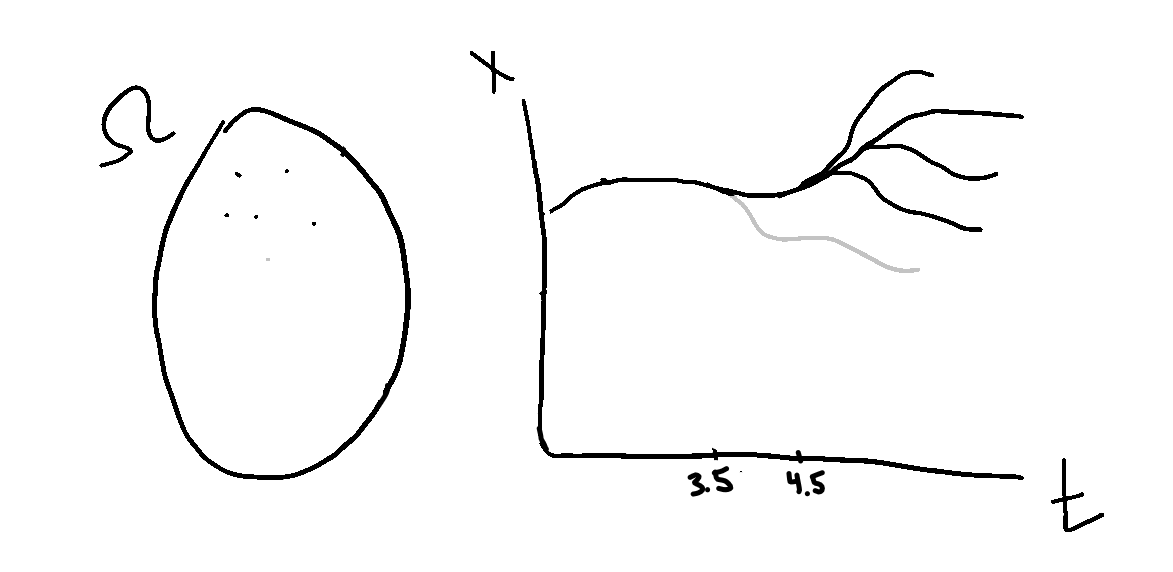
\includegraphics[width=\textwidth]{Filtration_grayed_4.5.png}

And it is hard to see, but one of the elements in the sample space is also grayed out. Which leaves us with our final image of $X_t(4.5)$:

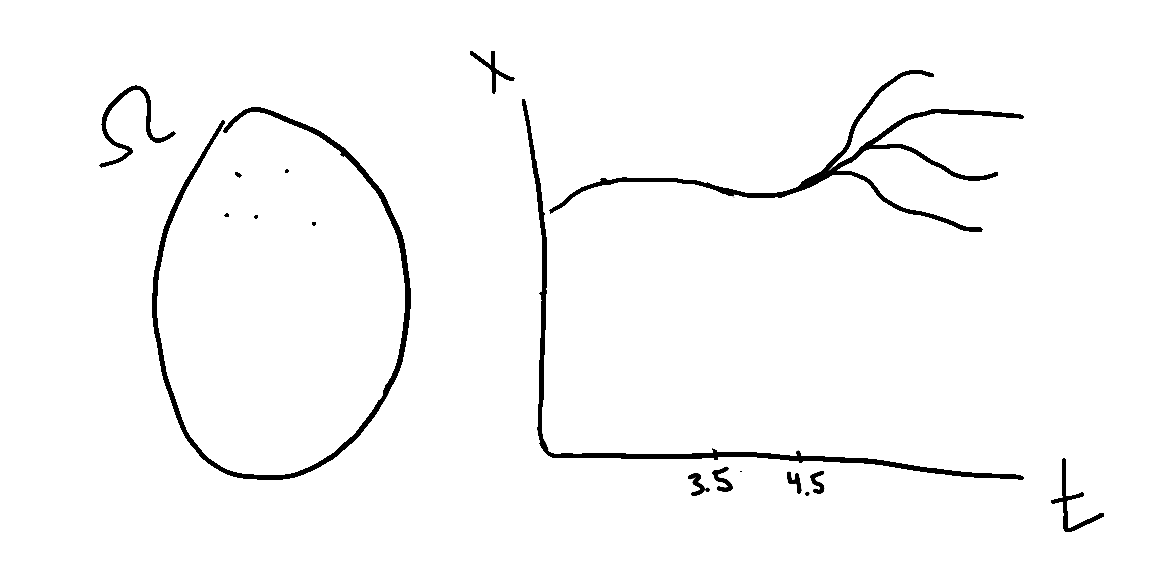
\includegraphics[width=\textwidth]{final_4.5.png}

And this time, it's very clear that I miscounted, and there should only be four elements in the sample space corresponding to the four possible trajectories.





\section{Differentiation and Integration}
Here is the best way I know to think about stochastic differentiation and integration. We'll redraw our picture, and its equation and notation are given below.

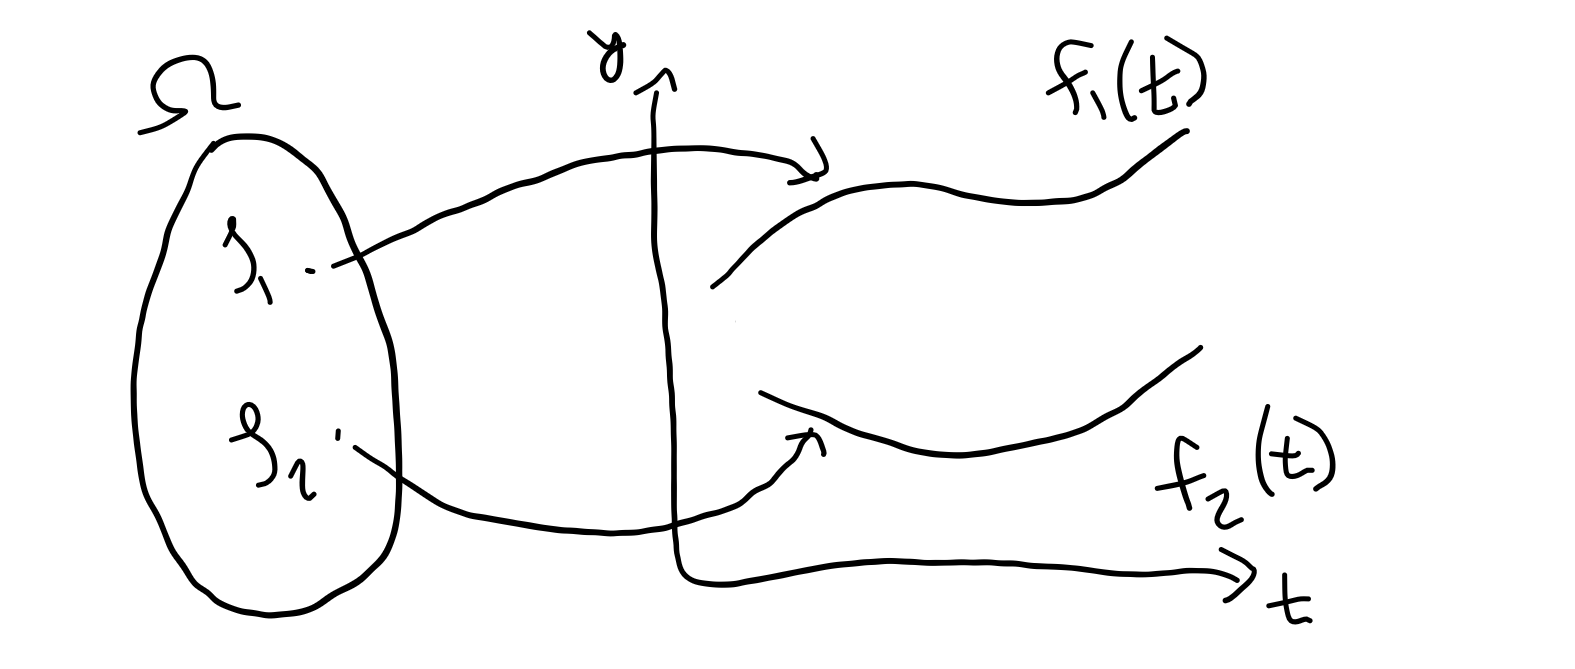
\includegraphics[width=\textwidth]{stochastic_ image.png}

$$X_t = x : \Omega \rightarrow \left(\mathbb{R}^+ \rightarrow  \mathbb{R} \right)$$ 
$$x(\varsigma_1) = f_1(t)$$
$$x(\varsigma_2) = f_2(t)$$
$$x(\varsigma) = f_\varsigma(t)$$

And note that $x$ is simply a deterministic function.  Also note that we can partially apply and curry however we want, so we also have the following, which will be useful in the following section:

$$X_t = x : \Omega \rightarrow \left(\mathbb{R}^+ \rightarrow  \mathbb{R} \right) = \Omega \rightarrow \mathbb{R}^+ \rightarrow  \mathbb{R} = x :  \left(\Omega  , \mathbb{R}^+\right)\rightarrow  \mathbb{R}$$ 

\subsection{Differentiation}
We have that:

$$X_t' = \frac{\partial}{\partial t}x(\varsigma,t)= \frac{x\left(\varsigma, t + h\right) - x\left(\varsigma, t\right)}{h} = \frac{f_\varsigma\left(t + h\right) - f_\varsigma\left(t\right)}{h} = \frac{df_\varsigma}{dt} =g\left(\varsigma, t\right)$$

Which means that $X_t'$ is just the probability weighted derivatives of the trajectories. Which, just like $x$, is just a deterministiic function of $\varsigma$ and $t$

Side note that this does not work in Brownian Motion because the individual trajectories in Brownian Motion are not differentiable (anywhere).  I think we might be able to do it with some form of a weak derivative, though, just not the regular one.

Also note that we are using the prime notation for a derivative, but it is a partial derivative. That's okay because $\Omega$ isn't necessarily a continuous variable like $t$ is, so when we're differentiating, it is understood that we're differentiating with respect to the only reasonable option, $t$.

\subsection{Integration}
We have that:
$$\int X_t= \int_{s = 0}^{s = t} X_s ds = \int_{s = 0}^{s = t} x\left(\varsigma,s\right) ds = \int_{s = 0}^{s = t} f_\varsigma\left(s\right) ds  = h\left(\varsigma,t\right)$$

Which means that $\int X_t$ is just the probability weighted integrals of the trajectories.  Which, just like $x$ and $g$, is just a deterministic function of $\varsigma$ and $t$

I think we can do this with Brownian Motion because even though Brownian Motion trajectories are not (in the normal sense) differentiable, they are integrable.

\subsection{Differentiation and Integration Example}
Suppose there are only two states of the world, Heads and Tails.  And if Heads is flipped, our world is $x^2 + 2$ and if Tails is flipped, we get $1$.  Our process is:

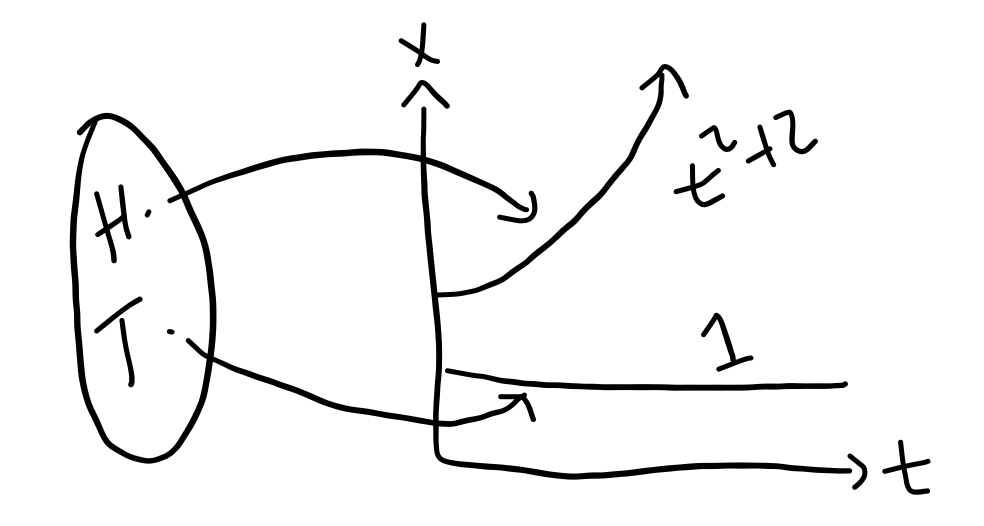
\includegraphics[width=\textwidth]{ExampleProcess.png}

\[X_t = \begin{cases} 
    t^2 + 2 & H \\
    1 & T 
 \end{cases}
\]

Then we also know:

\[\int X_t = \begin{cases} 
    \frac{1}{3}t^3 + 2t + C_1 & H \\
    t + C_2 & T 
 \end{cases}
\]
\[X_t = \begin{cases} 
    t^2 + 2 & H \\
    1 & T 
 \end{cases}
\]
\[X'_t = \begin{cases} 
    2t & H \\
    0 & T 
 \end{cases}
\]

And those integration constants are deterministic (i.e. they are just numbers).

\end{document}
